\section{Introduction}

Previous high speed ISR/camera data fusion efforts have used a single high-speed camera \citep{semeter2008,akbari2013,dahlgren2013}.
Auroral tomography with multiple cameras and ISR has previously been accomplished at low speed \citep{bjornthesis,wedlund2013}.
Studies of the aurora using two or more cameras with overlapping fields of view (FOV) were carried out in earnest from 1910 onward \citep{stormer1930}.
More recent work focused on the formal application of tomographic techniques \citep{frey1996,doe1997,bjorn1998,semeter1999,hirsch2016}.
Auroral tomography provides a means of accessing time-dependent information about remote auroral acceleration processes.
In this technique, common volume measurements of the aurora from multiple ground-based imagers are used to reconstruct the wavelength-dependent ionospheric volume emission rate (VER).
VER depends on the energy flux distribution of the precipitating magnetospheric electrons that have undergone a particular acceleration process, gaining high enough energy to penetrate deep into the ionosphere, giving rise to the auroral emissions via collisional and kinetic interactions with neutral species and ions.
The VER reconstruction is used together with a physics-based model of precipitating magnetospheric electrons to estimate the spatial distribution and characteristic energy of the primary electron differential number flux.
Estimation and measurements of the precipitation characteristic energy have been used \citep{chaston2003,mcfadden1999} as a conduit to understand mechanisms driving auroral morphology at the finest spatiotemporal scales.
Figure~\ref{fig:priortomo} represents the relation of prior work in this field to the advances made in this dissertation in Figure~\ref{fig:thistomo}.
The ability of the HiST system to simultaneously obtain estimates of precipitating flux characteristics vs. time \textit{and} space \citep{hirsch2016} are necessary to characterize the evolution of dispersive Alfvén waves in the lower magnetosphere accelerating electrons that cause the microstructure seen in the lower ionospheric aurora \citep{semeter2012}.
\begin{figure}\centering 
    %the \par is necessary after each text to make the \baselineskip take effect
    \begin{tikzpicture}[node distance=1.5cm, auto]
    
    \node (phi) [startstop,text width=5cm] {$\Phi_{top}(E,t,x)$ dispersive precipitating electron flux \par};
    
    \node (ver) [process, below of=phi,text width=2.5cm,xshift=2.5cm] { Structured Aurora \par };
    \node (turb)[process, left of=ver, text width=3.5cm,xshift=-2.5cm]{ Lower Ionospheric Plasma Turbulence \par};
    
    \node(isr) [process, below of=turb, text width=3cm] { ISR: strong backscatter \par};
    
    \node (onecam) [process, below of=ver, text width=2.5cm] { single camera \par };

	\node (oneinv) [compute, below of=onecam,text width=3cm] { Estimate $\widehat{\Phi}_{top}(E,t)$ \par};
    
    \draw[arrow] (phi) -- (turb);
    \draw[arrow] (turb)--(isr);
    \draw[arrow] (isr)|-(oneinv) node[pos=0.85, above] {$z_0, N_e$};
    
    \draw[arrow] (phi) -- (ver);
    \draw[arrow] (ver) -- (onecam);
    \draw[arrow] (onecam) -- (oneinv);

    
    \end{tikzpicture}
    
    \caption{Prior work in single camera, single flux tube precipitating electron flux estimation vs. time.}
    \label{fig:priortomo}
\end{figure}

\begin{figure}\centering 
	%the \par is necessary after each text to make the \baselineskip take effect
	\begin{tikzpicture}[node distance=1.5cm, auto]
	
	\node (phi) [startstop,text width=5cm] {$\Phi_{top}(E,t,x)$ dispersive precipitating electron flux \par};
	
	\node (ver) [process, below of=phi,text width=2.5cm,xshift=2.5cm] { Structured Aurora \par };
	\node (turb)[process, left of=ver, text width=3.5cm,xshift=-2.5cm]{ Lower Ionospheric Plasma Turbulence \par};
	
	\node(isr) [process, below of=turb, text width=3cm] { ISR: strong backscatter \par};
	
	\node (cam) [process, below of=ver, text width=2.5cm] { multiple cameras \par };
	
	\node (caminv) [compute, below of=onecam,text width=3cm] { Estimate $\widehat{\Phi}_{top}(E,t,x)$ \par};
	
	\draw[arrow] (phi) -- (turb);
	\draw[arrow] (turb)--(isr);
	\draw[arrow] (isr)|-(caminv) node[pos=0.9, above] {$N_e$};
	
	\draw[arrow] (phi) -- (ver);
	\draw[arrow] (ver) -- (cam);
	\draw[arrow] (cam) -- (caminv);
	
	
	\end{tikzpicture}
	
	\caption{Thesis work in multi-camera precipitating flux estimation vs. time and space.}
	\label{fig:thistomo}
\end{figure}


The reconstruction problem of Figure~\ref{fig:thistomo} is challenging owing to uncertainties in model assumptions and the solution non-uniqueness that arises from the constrained viewing geometry.
The use of a first-principles based physics model was motivated in part by the limited observation in the direction along the geomagnetic field $B_\parallel$.
The short distance between cameras was motivated by the desire to get the highest feasible resolution in the direction perpendicular to the geomagnetic field $B_\perp$ as simulated in Figure~\ref{fig:camres}.
These data inversion techniques provide the first realizable method of obtaining a persistent two-dimensional (energy, $B_\perp$) high resolution morphology estimate of the rapidly evolving electron precipitation above the ionosphere at the smallest ground-observable scales.

Auroral morphologies can be described in a Cartesian coördinate system, with axis $B_\parallel$ oriented along the Earth's local magnetic field $B$.
The HiST phase 1 system was deployed on Poker Flat Research Range (PFRR) with the configuration of Figure~\ref{fig:histloc}.
\begin{figure}
	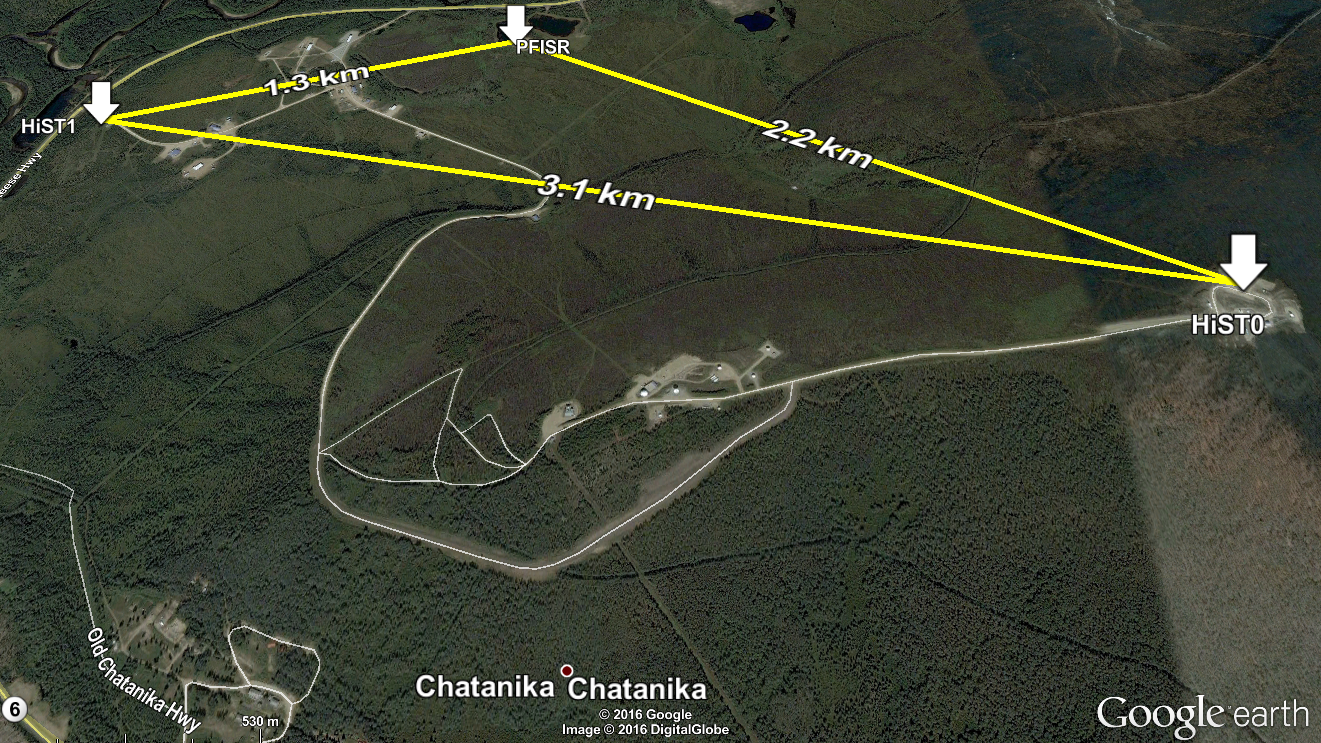
\includegraphics[width=\linewidth,trim=0 360 0 0,clip]{gfx/3sites}
	\caption{Location of HiST and PFISR at PFRR, Chatanika, AK. PFRR (65.1$^\circ$N, -147.5$^\circ$W) is \unit[30]{km} N-NE of Fairbanks, AK.}\label{fig:histloc}
\end{figure}
At PFRR, the inclination of the E-layer magnetic field is $77.5^\circ$, so the $B_\parallel$ axis is tipped $12.5^\circ$ from the local geographic vertical axis toward magnetic south.
The $B_\perp$ axis is defined to be orthogonal to $B_\parallel$ and coplanar with the cameras.
In auroral literature the ``width'' of auroral features refers to extent in the $B_\perp$ direction, and we follow this convention.

Prior work in auroral tomography \citep{jones1991,semeter1999,frey1998} has focused almost exclusively on mesoscale features of $\unit[10^4]{m}$ width recorded with typical sampling periods of order 1..\unit[30]{s}, with sensor baselines of 50..\unit[150]{km}.
The peak auroral emission intensity typically lies in the altitude range of approximately 100..\unit[300]{km}.
The $B_\parallel$ profile of the arc is dependent on the electron beam differential number flux and the characteristics of the neutrals and ions with which the precipitating particles interact.
An active auroral display embodies a vast hierarchy of spatial scales.
The global auroral oval is of order $\unit[10^5]{m}$ width as measured along magnetic latitude from the poleward to equatorward edges.
Dynamic fine-scale features embedded in an auroral breakup of $\unit[10^2]{m}$ width are typically observed during the substorm expansion phase \citep{semeter2008}.
Anthropogenic aurora of $\unit[10^2]{m}$ width has been observed from HAARP stimulus \citep{pederson2010,kendall2010}.
A complete theory of the aurora must account for variations at all scales inherent in the phenomena.
Although our theoretical understanding of global and mesoscale variability, and its drivers in the solar wind and magnetosphere, is well developed \citep{borovsky1993}, the physics underlying decameter-scale structure embedded within active auroral displays remains incomplete.

Auroral structures of sub-\unit[100]{m} width have been known to exist for decades \citep{maggsdavis1968,trondsendis}, and are seen regularly in long-term observations with modern cameras.
An example of a thin \unit[100]{m} wide auroral structure exhibiting rapid lateral motion is shown in the image sequence of Figure~\ref{fig:perspTrans}.
Note the substantial change in appearance of the arc in $1.5$ seconds, corresponding to a $5^\circ$ change in observer perspective, or about \unit[10]{km} in the $B_\perp$ dimension assuming \unit[120]{km} apparent auroral feature altitude.
%
An example of flaming aurora \citep{omholtbook,dahlgren2013} evolving over \unit[600]{ms} is shown in Figure~\ref{fig:perspFlame}.
%Both of these examples were recorded during the expansion phase of an auroral substorm.
%
% X1387_032307_112015.36_full_30fps.avi
% convert -normalize X1387*.avi[1132] 1132.png
% convert -normalize X1387*.avi[1147] 1147.png
% convert -normalize X1387*.avi[1162] 1162.png
% convert -normalize X1387*.avi[1177] 1177.png
% montage anno_11*.png -trim -tile 4x1 -geometry +1+0  anno_trans.png
\begin{figure*}\centering
    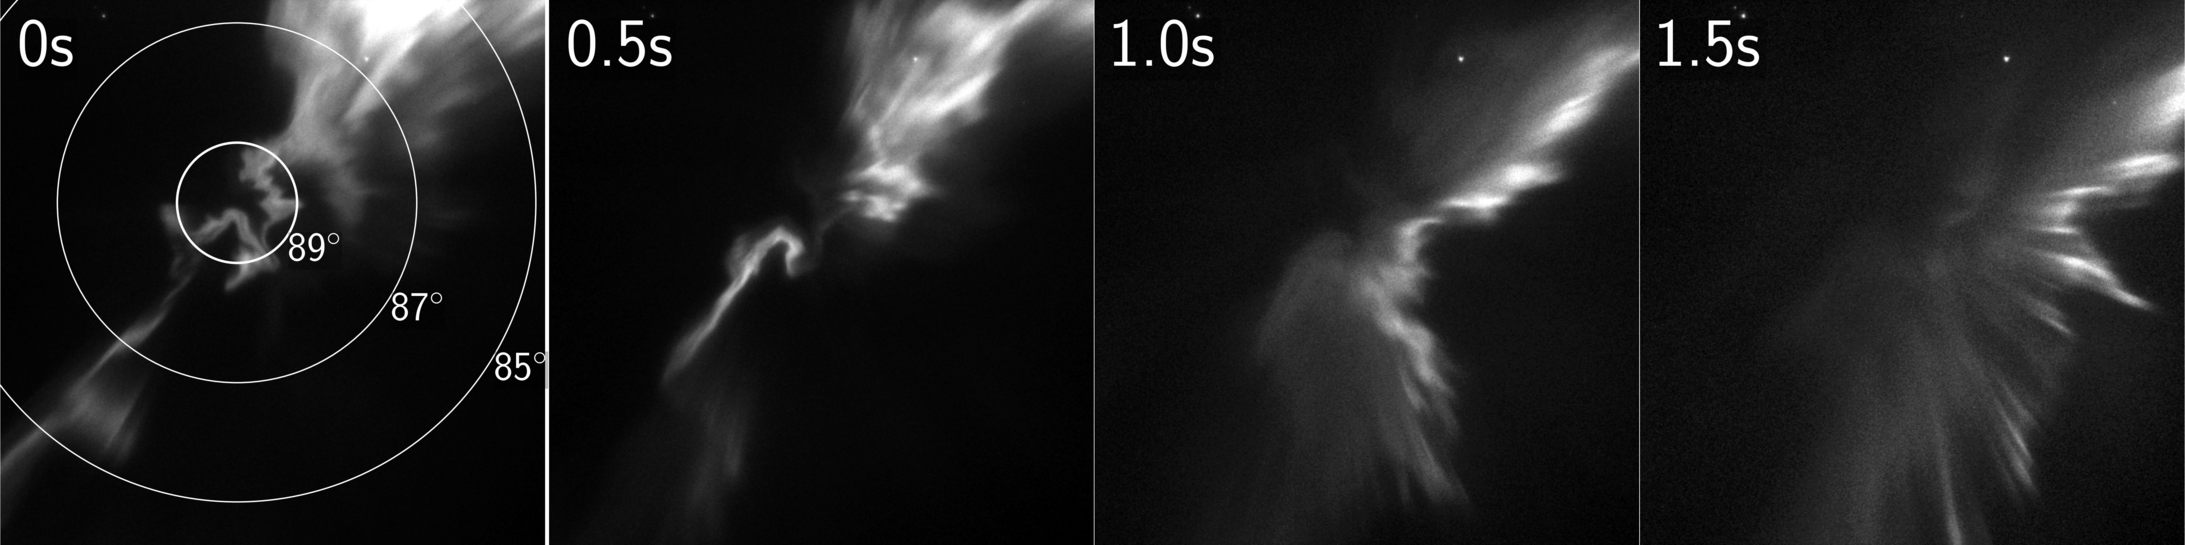
\includegraphics[width=\textwidth]{gfx/2007-03-23breakup}
    \caption{Radical change in perspective for \unit[100]{m} structure in \unit[1.5]{s} due to apparent $B_\perp$ transverse motion \citep{semeter2012,semeter2008}. 
    Contours are centered on local magnetic zenith.}
	\label{fig:perspTrans}
\end{figure*}
%
% generate figure 2.
%
% convert /tmp/CMOSvideo-0223.png -crop 900x550+880+610 flame100615440.png
% convert /tmp/CMOSvideo-0233.png -crop 900x550+880+610 flame100615640.png
% convert /tmp/CMOSvideo-0243.png -crop 900x550+880+610 flame100615840.png
% convert /tmp/CMOSvideo-0253.png -crop 900x550+880+610 flame100616040.png
% python fiducial.py
% montage anno_flame10061*.png -trim -tile 4x1 -geometry +1+0  anno_flame.png
%
%
\begin{figure*}\centering
    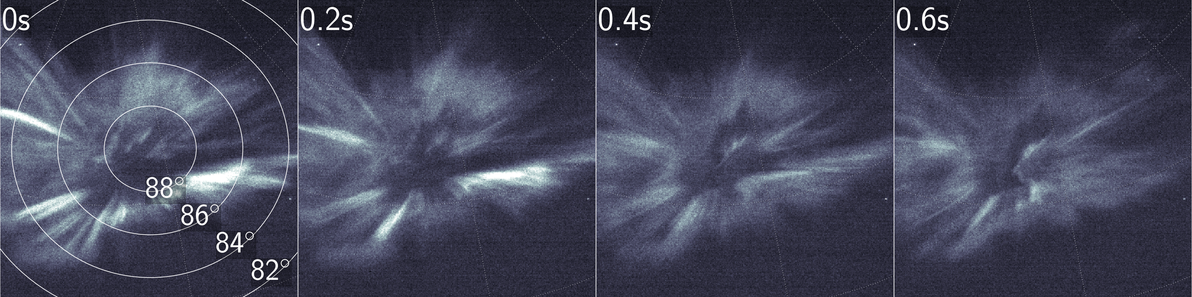
\includegraphics[width=\textwidth]{gfx/2011-03-01flame}
    \caption{Flaming aurora evolution over \unit[600]{ms} \citep{dahlgren2013}.
             Contours are centered on local magnetic zenith.}
    \label{fig:perspFlame}
\end{figure*}

Auroral acceleration occurs mainly in the altitude regime from 1000..\unit[40000]{km} \citep{lysak2011}, with DAW acceleration occurring mainly in the 1500..\unit[7000]{km} altitude range \citep{semeter2012}.
While the techniques of this system do not directly measure the acceleration regime, they do measure the outcomes of the acceleration.
The physics model based iterative reconstruction employed allows reconstructing particle flux at \unit[1000]{km} altitude, below which particle acceleration is negligible.
The reconstruction occurs over a sufficiently wide swath of sky (and can be widened by adding more cameras) to help characterize DAW structure in the lower magnetosphere.
%TODO block diagram showing magnetosphere

The tomographic techniques described in this dissertation contribute to understanding how such ephemeral fine-scale structure emerges in the incoming particle flux.
The observational requirements for a tomographic imaging system capable of resolving these scales are extreme, and the resulting inverse problem is highly ill-conditioned.
Section~\ref{sec:hist} presents the High Speed Tomography system (HiST) hardware \citep{hirsch2016}.
Sections~\ref{sec:flame} and~\ref{sec:transverse} comprise a feasibility study for a high frame-rate, short baseline, auroral tomography system.
Through simulation and modeling, we demonstrate that Electron Multiplying CCD (EMCCD) camera technology coupled with a physics-based regularization scheme is capable of resolving electron differential number flux dynamics of order \unit[100]{m} and \unit[10]{ms}.
The highest sensitivity cameras especially suitable for weak filtered auroral emissions are EMCCD-based.
EMCCD cameras are the core of the HiST system, along with GPSDO synchronization and embedded vision algorithms.
